% !TEX TS-program = LuaLaTeX

\documentclass[11pt,compress,xcolor=x11names,UTF8]{beamer}
\usetheme{Boadilla}
\usecolortheme{seahorse}
\useinnertheme[shadow]{rounded}
\useoutertheme[subsection=false]{smoothbars}
\usecolortheme{spruce}
\usecolortheme[named=SpringGreen4]{structure}
\usefonttheme{structurebold}
\useinnertheme{circles}
\usecolortheme{rose}
\usepackage{pifont}
\usepackage{academicons}
\usepackage{fontawesome}
\usepackage{iitem}
\usepackage{graphicx}
\usepackage{tabularx}
\setbeamertemplate{itemize item}{\ding{108}}
\setbeamertemplate{itemize subitem}{\ding{109}}
\setbeamertemplate{navigation symbols}{}
\setbeamercovered{transparent}
\renewcommand\appendixname{附录}
\renewcommand\abstractname{摘要}
\graphicspath{{figure/}} % 图片路径
\usepackage{calligra} % Thank you
\usepackage{ctex} % 加入中文
%\setCJKsansfont{Noto Sans CJK SC}
%\setsansfont{DejaVu} % Lato Roboto Fira Sans
\setsansfont{Lato} % Lato Roboto Fira Sans
\usepackage{makecell}
\newcommand{\tabincell}[2]{\begin{tabular}{@{}#1@{}}#2\end{tabular}}
\usepackage{url}
\usepackage{natbib} % 参考文献
%\title[Spatial Generalized Linear Mixed Models]{Spatial Generalized Linear Mixed Models with Application to Prevalence Mapping}
\title{ Converting  the PMT Container Testing Raw Data to ROOT File Format}
%\subtitle{奖助金申请答辩}
\author[Rong Zhao]{Email:zhaor25@mail2.sysu.edu.cn \and  } % \\ 专业:统计学 \\ 方向:数据分析与统计计算
\institute[SYSU]{School of Physics\and } % 理学院\\
\date[\today]{\includegraphics[width=.5\textwidth]{logo}}

\begin{document}

\maketitle

\begin{frame}{Outline}
\tableofcontents
\end{frame}


\section{converting raw data to root file}
\begin{frame}{ motivation}
%\textsf{例} \textbf{例}  \textit{例}
% \texttt{例}  % 调出仿宋字体了
%\begin{table}[]
%\caption{PMT performance qualification standard}
%\resizebox{.8\textwidth}{!}{%
%\begin{tabular*}{.98\textwidth}{l|c|c}
%%\toprule
%\hline
%\hline
%parameter & HAMAMATSU PMT&NNVT PMT\\
%\hline
%HV@Gain=$10^7$ &  <2350 V&<2800V \\
% PDE & >24\%& >24\%\\
% DCR & <50kHz& <100kHz\\
% PV & >2.5& >2.5\\
% rise time & <8.5ns& --\\
% fall time & <12ns&-- \\
% FWHM & ----& --\\
% resolution & <0.4&<0.4 \\
%\hline
%\end{tabular*}
%}
%\end{table}
\begin{enumerate}
\item 	The Raw data of PMT testing is significant for the evaluation of PMT performance. 
\item \textbf{While,Currently, the raw data of container system is not well organized and it is  not convinent for people to get a quikly access.  }
\item \alert{It is useful to convert all the testing raw data to ROOT format.}
\begin{itemize}
\item decrease the file size
\item easy to analysis and manage.
\item shadow the hardware details.
\end{itemize}
\end{enumerate}
%\begin{figure}
%\centering
%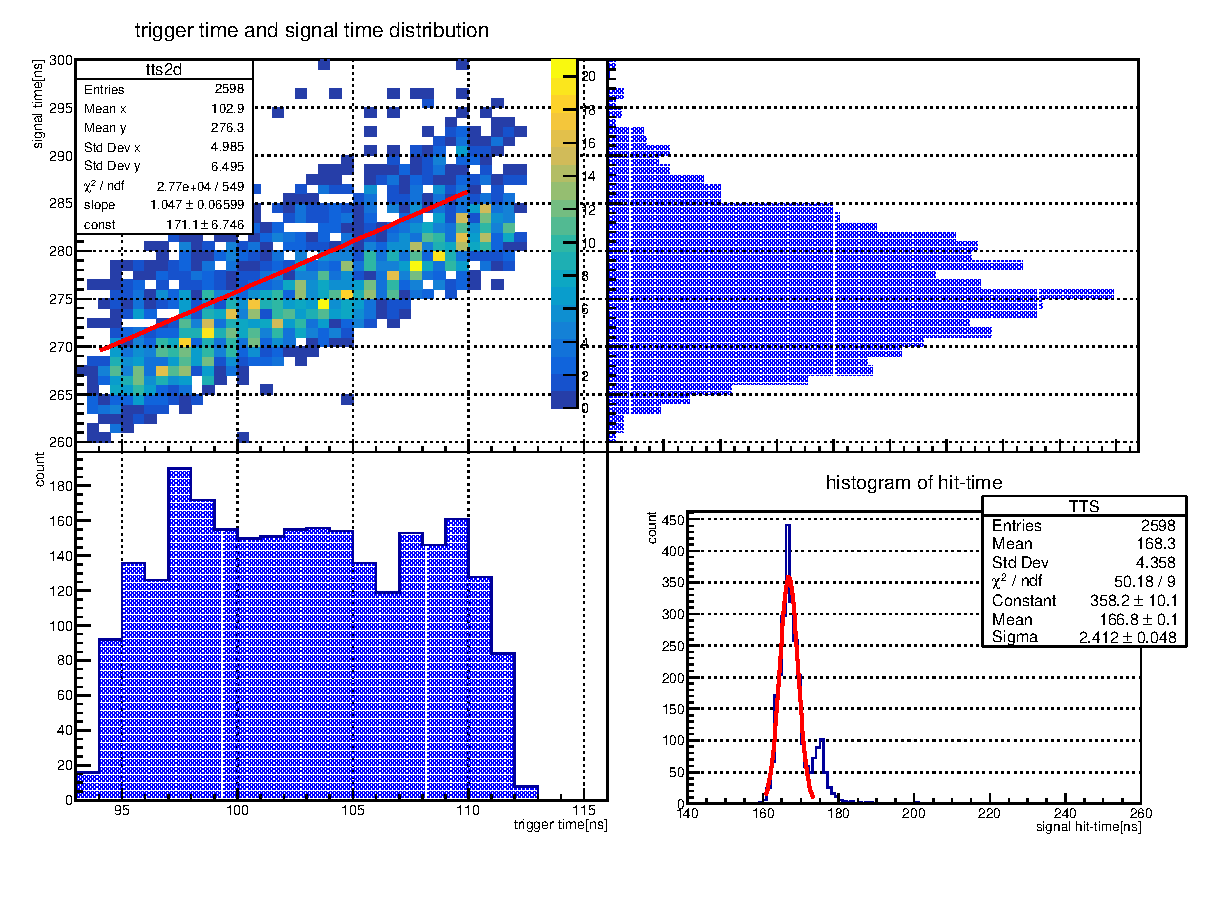
\includegraphics[width=0.78\textwidth]{typical_hittime} % 单图
%\end{figure}
\end{frame}
%%%%%%%%%%%%%%%%%%%%%%%%%%%%%%%%%%%%%%%%%%%
\begin{frame}{requirements}
\begin{enumerate}
\item sotre the raw waveform data(.1pe, 1pe, TTS).
\item store the auxilary testing information(container #, mass#, HV, DCR. etc).
\item easy to manage (create, modify and update) and analyze.
\item \alert{one ane acquire almost all the data needed for analysis(of one PMT) from only one file} rather than collecting the details from server.

\end{enumerate}
\end{frame}
%%%%%%%%%%%%%%%%%%%%%%%%%%%%%%%%%%%%%%%%%%%
\begin{frame}{prliminary file structure and strategies}
\begin{itemize}
\item each PMT have one root file named in "SN\_rawdata.root"
\item In a specific root file, we have several waveform waveform trees and a auxilary data tree
\item if one PMT go through several tests in the container, all the data will be saved still in only one root file but with different name of wave trees\footnote{distiguished by a unique tag}; their auxilary information will be filled several times in the same tree. 
\end{itemize}
\begin{figure}
\centering
\includegraphics[width=0.98\textwidth]{figures/tree.png} % 单图
\end{figure}

\end{frame}
%%%%%%%%%%%%%%%%%%%%%%%%%%%%%%%%%%%%%%%%%%%
\begin{frame}{ restore the waveforms}
all the aveforms were stored as a vetor with 521 length, one can easily read and analysis the data, for example : 
\begin{figure}
\centering
\includegraphics[width=0.98\textwidth]{figures/exam.png} % 单图
\end{figure}

\end{frame}
%%%%%%%%%%%%%%%%%%%%%%%%%%%%%%%%%%%%%%%%%%%
\begin{frame}{ current states}
%current file path:
%the folder MCP contains all the MCP PMT data files;
%the folder HAMAMATSU contains all the  HAMAMATSU data files;
finished:
\begin{itemize}
\item basic structure of root file and TTree
\item example rawdata root file
\item example cpp program to access the waveforms from the generated root file
\end{itemize}
still working on :
\begin{itemize}
\item refine the root file contents and structure
\item writing the doucument for potential users
\end{itemize}
 
\end{frame}
%%%%%%%%%%%%%%%%%%%%%%%%%%%%%%%%%%%%%%%%%%%
%\begin{frame}{calibration of each drawer}
%Generally, we put several PMTs with known PDE value\footnote{or QE value}  into one drawer and linearly fit the PDE-$\mu_{test}$ data to get \alert{drawer$_{factor}$}.
%\vspace{.5cm}
%\hrule{\textwidth}
%\vspace{.5cm}
%
%While an alternative way to access the drawer$_{factor}$ is fitting PDE-$\mu_{test}$ data {\color{red}from all the PMTs tested in one drawer rather than the mannual selected ones.} Then once we finish one PMT test in a drawer we will get one more statistical sample in the PDE-$\mu_{test}$ fitting, and we could expect that the fitted drawer$_{factor}$ will get more stable as we testing more PMTs.
%
%\vspace{.5cm}
%The advantage of this "self-calibration" method is that we could {\color{red}decrease the statistical error as much as possible}; and the remained fluctuation of drawer$_{factor}$ can be the system error.
%\end{frame}
%\section{Waveform and Charge Spectrum}
%%%%%%%%%%%%%%%%%%%%%%%%%%%%%%%%%%%%%%%%%%%
%\begin{frame}{抽屉刻度方法}
%滨松厂家提供部分PMT的QE\footnote{假定所有的PMT的收集效率相同}值,可以从PMT数据库\footnote{王俊[http://pmtdb.juno.ihep.ac.cn/index.html]}查询到。如果某一个抽屉测到的滨松PMT恰好有QE的厂家值,就选用它进行刻度。
%
%\vspace{.5cm}
%\hrule{\textwidth}
%\vspace{.5cm}
%为了保证刻度PMT的性能,只选取通过集装箱测试的PMT进行刻度。
%\end{frame}
%%%%%%%%%%%%%%%%%%%%%%%%%%%%%%%%%%%%%%%%%%%
%\begin{frame}{一个抽屉的刻度结果}
%随着测试PMT数量的增加,拟合统计误差逐渐减小,$drawer_{factor}$的拟合结果趋于稳定(更多抽屉拟合结果见back-up部分)。
%\begin{figure}
%\centering
%\includegraphics[width=0.98\textwidth]{sta101-7} % 单图
%\caption{108抽屉的$drawer_{factor}$拟合结果}
%\end{figure}
%\end{frame}
%%%%%%%%%%%%%%%%%%%%%%%%%%%%%%%%%%%%%%%%%%%
\section{update of container test results}
\begin{frame}{updates from shanghai colaberation meeting}
\end{frame}
%%%%%%%%%%%%%%%%%%%%%%%%%%%%%%%%%%%%%%%%%%%
%%%%%%%%%%%%%%%%%%%%%%%%%%%%%%%%%%%%%%%%%%%%%%%%%%%%%%
\section{Summary}

\begin{frame}{summary}
\begin{itemize}
\item the converting of raw data from binary to root format is almost done  
\item one can easily restore the test waveforms with no loss of information
\item  the file size\footnote{the total additional disk space requirement for 20k is less than 2T, so this not a problem} decrease about 20\% after transform\footnote{about 50MB for one PMT of one light intensity}.
%\item  {\color{red}we need to study the "delay signal" of HAMAMATSU PMT and "big signal" of NNVT PMT\footnote{especially when PMT working in the multi-photon case}} in detail\footnote{one option is to transport several PMTs to SYSU for detailed study}.
\item the update of container results
%\item 保存重要的测试信息和输出结果到PMT数据库,所有测试结果\footnote{包含集装测试历史数据}可以直接通过http://pmtdb.juno.ihep.ac.cn/\footnote{Query::LPMT Tested Reports} 查询得到
%\item 初步结论:目前现场5002支滨松PMT,382支外观检测不合格,5支HV不合格,2支波形较差,24支DCR不合格,9支PDE不合格。
\end{itemize}
\end{frame}

\begin{frame}
\centering {\zihao{0} \color{red} {THANKS}}
\end{frame}

\begin{frame}
\centering {\zihao{0} \color{red} {BACK-UP}}
\end{frame}

%\begin{table}[htbp]
%\caption{PMT typical performance}
%\resizebox{.8\textwidth}{!}{%
%\begin{tabular*}{.98\textwidth}{l|cccc}
%%\toprule
%\hline
%\hline
%Performance & PDE &DCR & TTS& uniformity \\
%\hline
%HAMAMATSU &  lower\% & 20 kHz& 3ns& worse \\
%NNVT  & higher\% & 40kHz & 7ns& better \\
%\hline
%\end{tabular*}
%%}
%\end{table}

%\end{frame}
%%%%%%%%%%%%%%%%%%%%%%%%%%%%%%%%%%%%%%%%%%%%%%%%%%%%%%
\begin{frame}{TTS of HAMAMATSU PMT}
\begin{figure}
\centering
\includegraphics[width=.8\textwidth]{figures/hamtts.JPG} % 单图
%\label{fig:wave2d}
\caption{hittime and trigger time}
\end{figure}
\end{frame}
%%%%%%%%%%%%%%%%%%%%%%%%%%%%%%%%%%%%%%%%%%%%
%%%%%%%%%%%%%%%%%%%%%%%%%%%%%%%%%%%%%%%%%%%%%%%%%%%%%%%%%%%%%%%%%%%%

\appendix

\section*{附录}


\end{document}
